\chapter{Beispielanwendungen von Spark zur Datenanalyse}
Im Folgenden wird Apache Spark im Rahmen zweier grundsätzlich verschiedener Anwendungsfälle betrachtet. \\

Beispiel 1: Eine typische Anwendung mit verteilten lokalem Storage (HDFS) und Spark als "`Client"' eines bestehenden Yarn Clustermanagers. \textcolor{gray}{--- Commodity Hardware (Rasperry Pi Cluster). ---}\\


Beispiel 2: Eine untypische Anwendung mit verteiltem entfernten Storage und dem Spark Standalone Clustermanager. \textcolor{gray}{--- HPC Hardware ("`Thunder"' des Hamburger KlimaCampus). ---}\\

\section{Anwendung zur Echtzeitanalyse eines Datenstroms anhand eines veränderlichen Stammdatenbestandes}
\textcolor{gray}{--- Fusion von Tweets und Mailinglisten 
https://spark.apache.org/docs/1.3.0/mllib-feature-extraction.html
Implementation auf einem Raspberry Pi Cluster mit HDFS und Yarn Clustermanager ---}\\
\subsection{Problembeschreibung}
\textcolor{gray}{--- Es sollen die beiden Spark Mailingslisten (Developer, User) zur Identifikation relevanter und aktueller Themen genutzt werden. Mit den so bewerteten Begriffen können wiederum Tweets bewertet werden. Mit den Tweets können dann ganze Accounts nach ihrer Relevanz beurteilt werden. ---}\\
\textcolor{gray}{--- Zwei Datenquellen: Tweets (Nahe-Echtzeit), Entwickler-Emails (Sporadisch) ---}\\
\textcolor{gray}{--- Stichworte: HDFS, Yarn, Rasperri Pi Cluster, Machine Learning, Feature Extraction, Big Data Life Cycle ---}\\

Es sollen aktuelle Informationen bereitgestellt werden, die besonders für Nutzer und Entwickler des Softwareproduktes Apache Spark relevant sind.\\



\subsection{Anforderungen}

Für die Software soll folgende lose Sammlung funktionaler und nicht-funktionaler Anforderungen gelten. Mit \textit{Information} ist jeweils eine Auflistung von Twitter-Meldungen gemeint.

\begin{itemize}
	\item \textbf{A1: Zugriff auf die Information}\\
	Der Zugriff soll über eine grafische Benutzerschnittstelle erfolgen und keine Konfigurationen benötigen.
	\item \textbf{A2: Aktualität der Information}\\
	Es sollen stets Informationen dargestellt werden, die unmittelbar zuvor entstanden sind und in Quasi-Echtzeit\footnote{Eine Latenz von unter einer Minute sei hier tolerabel} verarbeitet wurden.
	\item \textbf{A3: Relevanz der Information}\\
	Die Relevanz soll an aktuellen Themen der Entwicklergemeinschaft gemessen werden.
\end{itemize}

\subsection{Hardwarekontext und Performance-Basisdaten}

Als Testumgebung dient ein \gls{cluster} aus vier identischen \gls{worker}n und einem speziellen \gls{master}knoten (Abb. \ref{figure:versuchsaufbau}).

\begin{figure}[h]
	\centering
  \includesvg[pdf]{versuchsaufbau}
	\caption{Hardwareumgebung des Programms zur Tweetanalyse}
	\label{figure:versuchsaufbau}
\end{figure}

\paragraph{Worker}
Rasperry Pi 2
\begin{itemize}
	\item CPU: 900MHz Quad-Core ARM Cortex A7
	\item RAM: 1GB SDRAM
	\item Ethernet: 100MBit/s
	\item Festspeicher: SDHC Class 4 Speicherkarte 16GB
\end{itemize}
Als Betriebssystem kommt das Debian-Derivat Raspbian\footcite{raspbian} 32-Bit zum Einsatz.

\paragraph{Master}
Dell d420
\begin{itemize}
	\item CPU: 1,2 GHz Core2 Duo U2500
	\item RAM: 2GB DDR2 SDRAM
	\item Ethernet: 100MBit/s
	\item Festspeicher: 60GB 4200RPM Hard Drive
\end{itemize}
Als Betriebssystem komm Ubuntu\footcite{ubuntu} 14.04 32-Bit zum Einsatz.

\paragraph{Netzwerk}
Vernetzt sind die Rechner mit \gls{rj45} über einen TP-Link TL-SF1008D Switch mit maximalem Durchsatz von 100MBit/s.

\begin{table}[ht]
\caption{---DUMMY--- Netzwerkdurchsatz} % title of Table
\centering % used for centering table
\begin{tabular}{c c c c} % centered columns (4 columns)
\hline\hline %inserts double horizontal lines
Nachrichtengröße & Worker $\rightarrow$ Worker & Master $\rightarrow$ Worker & Worker $\rightarrow$ Master \\ [0.5ex] % inserts table
%heading
\hline % inserts single horizontal line
1kB & 50ms & 837ms & 970ms \\ % inserting body of the table
64kB & 47ms & 877ms & 230ms \\
1MB & 31ms & 25ms & 415ms \\
64MB & 35ms & 144ms & 2356ms \\ [1ex] 
\hline %inserts single line
\end{tabular}
\label{table:nonlin} % is used to refer this table in the text
\end{table}

\subsection{Lösungsskizze}


\paragraph{Wahl des Dateisystems}

\textcolor{gray}{--- HDFS ---}\\

\paragraph{Wahl des Cluster-Managers}

\textcolor{gray}{--- YARN ---}\\

\paragraph{Verteilungsdiagramm}
\begin{figure}[h]
	\centering
  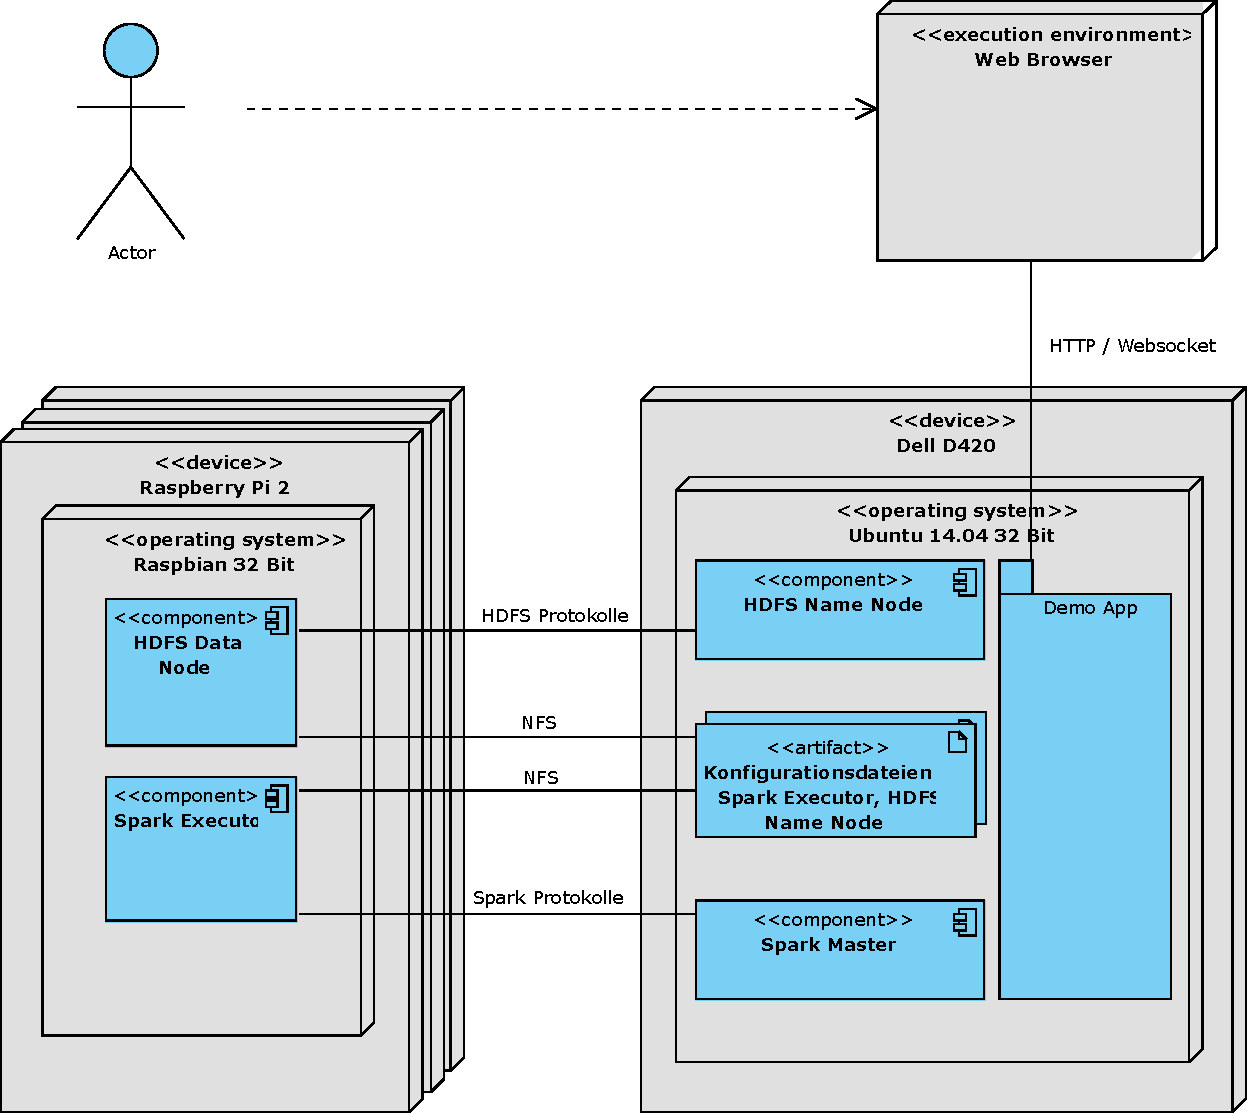
\includegraphics[scale=0.7]{demo_app_deployment.pdf}
	\caption{Verteilungssicht auf die Demo App}
	\label{figure:demo_app_verteilung}
\end{figure}

\paragraph{Komponentendiagramm}
\paragraph{Laufzeitdiagramme}

%\iffalse %%%%%%%%%%%%%%%%%%%%%%%%%%%%
\begin{center}
\begin{tikzpicture}
\begin{umlpackage}{Apache Spark}
\begin{umlcomponent}{A}
\umlbasiccomponent{B}
\umlbasiccomponent[y=-2]{C}

\umlrequiredinterface[interface=C-interface]{C}
\umlprovidedinterface[interface=B-interface, with port, distance=3cm, padding=2.5cm]{B}
\end{umlcomponent}
\umlbasiccomponent[x=-10,y=1]{D}
\end{umlpackage}
\umlbasiccomponent[x=3,y=-7.5]{E}
\umlbasiccomponent[x=-2, y=-9]{F}
\umlbasiccomponent[x=-7,y=-8]{G}
\umlbasiccomponent[x=-7,y=-11]{H}

\umlassemblyconnector[interface=DA, with port, name=toto]{D}{A}
\umldelegateconnector{A-west-port}{B-west-interface}
\umlVHVassemblyconnector[interface=AE, with port]{A}{E}
\umlHVHassemblyconnector[interface=EF, with port, first arm]{E}{F}
\umlHVHassemblyconnector[interface=GHF, with port, arm2=-2cm, last arm]{G}{F}
\umlHVHassemblyconnector[with port, arm2=-2cm, last arm]{H}{F}

\umlnote[x=-4, y=4, width=3.4cm]{B-west-interface}{Hier ist B-west-interface}
\umlnote[x=2, y=4, width=3.4cm]{C-east-interface}{Hier ist C-east-interface}
\umlnote[x=-8.5, y=-2, width=3.4cm]{toto-interface}{Hier ist toto-interface}
\umlnote[x=-5.5, y=-4.5, width=3.4cm]{A-south-port}{Hier ist A-south-port}
\umlnote[x=-1, y=-6, width=3.4cm]{AE-interface}{Hier ist AE-interface}
\umlnote[x=2, y=-11, width=3.4cm]{F-east-port}{Hier ist F-east-port}
\end{tikzpicture}
\end{center}

\textcolor{gray}{--- hier kommen diagramme und codeschnipsel hin ---}\\

\begin{lstlisting}[language=Scala, caption=Treiber für Testanwendung (Programmiersprache Scala)]
import org.apache.spark.SparkContext
import org.apache.spark.SparkContext._
import org.apache.spark.SparkConf

object ScalaApp {
  val my_spark_home = "/home/daniel/projects/spark-1.1.0"

  def main(args: Array[String]): Unit = {
    val logFile = my_spark_home + "/README.md"

    val conf = new SparkConf().setAppName("ScalaApp")
    val sc = new SparkContext(conf)

    val parList1 = sc.parallelize(List(1,2,3,4,5,6))
    val parList2 = sc.parallelize(List(5,6,7,8,9,10))
    val str1 = 
      "RDD1: \%s".format(parList1.collect().deep.mkString(" "))
    val str2 = 
      "RDD2: \%s".format(parList2.collect().deep.mkString(" "))
    val str3 = 
      "# of RDD1: \%s".format(parList1.count())
    val str4 = 
      "Intersect: \%s".format(parList1.intersection(parList2).collect()
    val str5 = 
      "Intersect: \%s".format(parList1.cartesian(parList2).collect()
  }
}
\end{lstlisting}

%%%%%%%%%%%%%%%%%%

\begin{center}
\begin{tikzpicture}
\begin{umlseqdiag}
\umlactor[class=A]{a}
\umldatabase[class=B, fill=blue!20]{b}
\umlmulti[class=C]{c}
\umlobject[class=D]{d}
\begin{umlcall}[op=opa(), type=synchron, return=0]{a}{b}
\begin{umlfragment}
\begin{umlcall}[op=opb(), type=synchron, return=1]{b}{c}
\begin{umlfragment}[type=alt, label=condition, inner xsep=8, fill=green!10]
\begin{umlcall}[op=opc(), type=asynchron, fill=red!10]{c}{d}
\end{umlcall}
\begin{umlcall}[type=return]{c}{b}
\end{umlcall}
\umlfpart[default]
\begin{umlcall}[op=opd(), type=synchron, return=3]{c}{d}
\end{umlcall}
\end{umlfragment}
\end{umlcall}
\end{umlfragment}
\begin{umlfragment}
\begin{umlcallself}[op=ope(), type=synchron, return=4]{b}
\begin{umlfragment}[type=assert]
\begin{umlcall}[op=opf(), type=synchron, return=5]{b}{c}
\end{umlcall}
\end{umlfragment}
\end{umlcallself}
\end{umlfragment}
\end{umlcall}
\umlcreatecall[class=E, x=8]{a}{e}
\begin{umlfragment}
\begin{umlcall}[op=opg(), name=test, type=synchron, return=6, dt=7, fill=red!10]{a}{e}
\umlcreatecall[class=F, stereo=boundary, x=12]{e}{f}
\end{umlcall}
\begin{umlcall}[op=oph(), type=synchron, return=7]{a}{e}
\end{umlcall}
\end{umlfragment}
\end{umlseqdiag}
\end{tikzpicture}
\end{center}
%\fi %%%%%%%%%%%%%%%%%%%%%%%%%%%%%%%%%%%%%%%%%%%%%%%%

\subsection{Ergebnisse und Bewertung}
\paragraph{Dashboard}
\paragraph{Laufzeitverhalten}
\paragraph{Bewertung und Probleme}


\section{Spark-basierte Implementation von Operatoren aus der Klimaforschung}
\textcolor{gray}{--- Implementation ausgewählter CDOs (sehr wenige, möglicherweise nur 1-2) mit der Core-API von Spark. Testlauf auf einem HPC Cluster mit nicht-lokalem, allerdings per Infiniband angeschlossenen Storage.
Insbesondere Betrachtung des Skalierungsverhaltens und der "`Sinnhaftigkeit"'. ---}

\subsection{Beschreibung des Problems}
\textcolor{gray}{--- Erläuterung von CDOs (Climate Data Operators). ---}
\subsection{Hardwarekontext und Performance-Basisdaten}
\textcolor{gray}{--- hier kommen die eingesetzten Systeme, und relevante Laufzeitmessungen (netzwerk, storage, cpu) hin ---}
\subsection{Architekturübersicht}
\textcolor{gray}{--- hier kommen Verteilungs- und Komponentendiagramm hin ---}
\subsection{Detailierte Lösungsbeschreibung}
\textcolor{gray}{--- hier kommen laufzeitdiagramme und codeschnipsel hin ---}
\subsection{Ergebnisse}
\textcolor{gray}{--- Tabellen und Diagramme Ergebnissen, evt. Skalierungsverhalten ---}
\textcolor{gray}{--- Bewertung ---}
